\chapter{Evaluation}

%In this chapter you should describe the previous (if possible) and final experiments performed on the implementation.

%Every single experiment should be explained individually, providing to the reader information about the meaning of the experiment, the expected %(theoretical) results, the final results, the comparison between them and others (if possible) and the conclusions. 

%Each experiment should include a description, covering (when possible) the following information:
%\begin{itemize}
%	\item Significant physical features (obstacles present on the environment, human presence, temperature, humidity, possible noise sources, computational speed of the machine, etc.)
%	\item The precise location of the experiment (latitude and longitude, room number or citation to a description of the used laboratory).
%	\item Sampling design (variable(s) measured, transformation performed to the data, samples collected, replication, comparative with a Ground Truth system, collecting data protocol).
%	\item Analysis design (how the data are processed, statistical procedures used, statistical level to determine significance).
%\end{itemize}
%The provided information should be sufficient to allow other scientists to repeat your experiment in the same conditions. Thus, the use of standard and %well-known equipment could only be represented by a simple sentence, but the non-standard equipment should be described in detail, citing the source %(vendor) and most important characteristics.

%To write it, try to use the third person when describing the experiments and results. Avoid to use first person. Past tense should be the dominant %conjugation (the work is done and was performed in the past).

%Note: Graphics represent really well data, use them! (Matlab or Octave could be useful for that).

\section{Experiment Setup}
To test the suggested approach for a RSS measurement system described in Chapter \ref{chp:apr} the approach was implemented like described in Chapter \ref{chp:imp}. System was then deployed and tested inside the Testbed described in Chapter \ref{chp:mat_testbed}. Two experiments where run. The first one was at night where no one was inside the building where the Testbed is located. The second one was at daytime when there where people where working inside the offices covered by the Testbed and also in the other parts of the building. 

The implemented system still had some bugs that could not be addressed due to lack of time. However these bugs only made the system stop at one point during the collection and did not influence the measured times for the different phases. This made it necessary to start the system multiple times for each experiment. The application was restarted after half an hour to catch stops. This however made it impossible to evaluate how long it takes until a new calibration is needed.

To calibrate the system 700 messages were sent. The timeslot for the drops was defined as 18 ms. This is really big but when running the system inside a simulation it could be measured that the processing and sending of a message took between 5 ms and 16 ms the extra 2 ms cover a possible error while measuring these values.  
\section{Experiment Night}
\begin{table}[htbp]
 \caption{Measured values for each run of the system. CT = Calibration Times; HOP = Number of hops inside the schedule; ST = Spread time; ACT = Average collection time; CSTD = Standard deviation of collection time; ART = Average round time; RSTD = Standard deviation of round time;}
 \centering
 \begin{tabular}{c||c|c|c|c|c|c|c|c}
  Time & CT & HOP & ST & ACT & CSTD & ART & RSTD & Rounds\\ \toprule
  02:00 - 02:30 & 65611 & 44 & 784 & 3592 & 267 & 540 & 55 & 338\\
  02:30 - 03:00 & 64545 & 42 & 842 & 3637 & 280 & 519 & 38 & 73\\
  03:00 - 03:30 & 64630 & 42 & 767 & 4211 & 444 & 502 & 32 & 13\\
  03:30 - 04:00 & 64539 & 41 & 740 & 3609 & 300 & 501 & 62 & 420\\
  04:00 - 04:30 & 64565 & 44 & 804 & 3581 & 245 & 544 & 51 & 419\\
  04:30 - 05:00 & 64699 & 40 & 756 & 4287 & 343 & 429 & 48 & 35\\
  05:00 - 05:30 & 64587 & 44 & 787 & 4150 & 343 & 496 & 23 & 9\\ \toprule
  Average & 64739 & 42 & 782 & 3738 & 290 & 518 & 48 & \\
 \end{tabular}
 \label{tab:NightTable}
\end{table}

\begin{figure}[htbp]
	\centering
	\begin{subfigure}[t]{1\textwidth}
		\centering
    		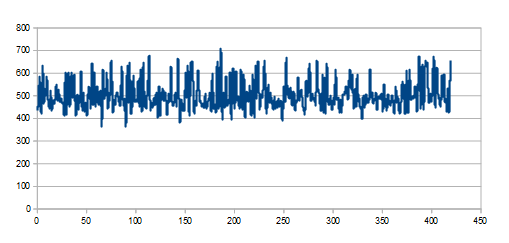
\includegraphics[scale=0.75]{content/images/Experiment/NightRounds}
   	 	\caption{Sampling times of the measurements from 03:30h to 04:00h}
    	\label{fig:nightR}
    \end{subfigure}
 
    \begin{subfigure}[t]{1\textwidth}
		\centering         
        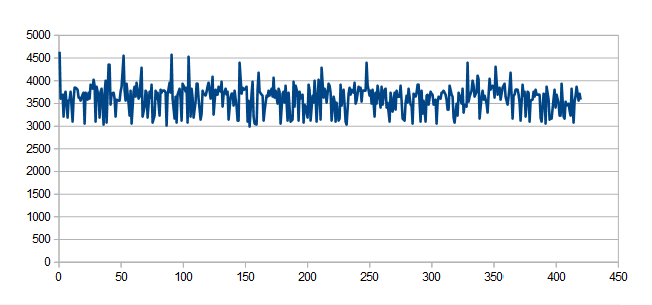
\includegraphics[scale=0.75]{content/images/Experiment/NightCollection}
        \caption{Collection times of the measurements from 03:30h to 04:00h}
        \label{fig:nightC}
    \end{subfigure}
    \caption{}
\end{figure}

\section{Experiment Day}
\begin{table}[htbp]
 \caption{Measured values for each run of the system. CT = Calibration Times; HOP = Number of hops inside the schedule; ST = Spread time; ACT = Average collection time; CSTD = Standard deviation of collection time; ART = Average round time; RSTD = Standard deviation of round time;}
 \centering
 \begin{tabular}{c||c|c|c|c|c|c|c|c}
  Time & CT & HOP & ST & ACT & CSTD & ART & RSTD & Rounds\\ \toprule
  09:15 - 09:45 & 64647 & 43 & 823 & 4401 & 296 & 492 & 41 & 63\\ 
  09:45 - 10:15 & 64558 & 44 & 796 & 4035 & 322 & 563 & 59 & 121\\
  10:15 - 10:45 & 64644 & 41 & 850 & 3740 & 282 & 482 & 40 & 231\\
  10:45 - 11:15 & 64577 & 41 & 849 & 3746 & 423 & 533 & 60 & 14\\ 
  11:15 - 11:45 & 64607 & 39 & 797 & 3498 & 358 & 495 & 42 & 433\\
  11:45 - 12:15 & 64654 & 41 & 764 & 3556 & 294 & 495 & 45 & 240\\
  12:15 - 12:45 & 64583 & 44 & 824 & 4160 & 511 & 539 & 65 & 368\\
  12:45 - 13:15 & 64544 & 44 & 797 & 3697 & 398 & 542 & 58 & 183\\
  13:15 - 13:45 & 64580 & 41 & 778 & 3494 & 371 & 528 & 46 & 73\\ \toprule
  Average & 64599 & 42 & 809 & 3773 & 372 & 514 & 50 & \\
 \end{tabular}
 \label{tab:NightTable}
\end{table}

\begin{figure}[htbp]
	\centering
	\begin{subfigure}[t]{1\textwidth}
		\centering
    		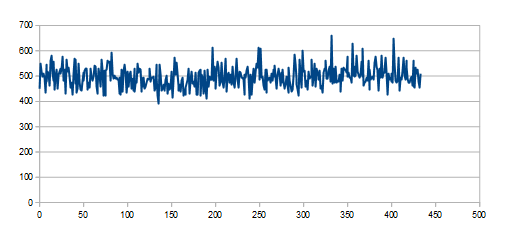
\includegraphics[scale=0.75]{content/images/Experiment/DayRounds}
   	 	\caption{Sampling times of the measurements from 03:30h to 04:00h}
    	\label{fig:DayR}
    \end{subfigure}
 
    \begin{subfigure}[t]{1\textwidth}
		\centering         
        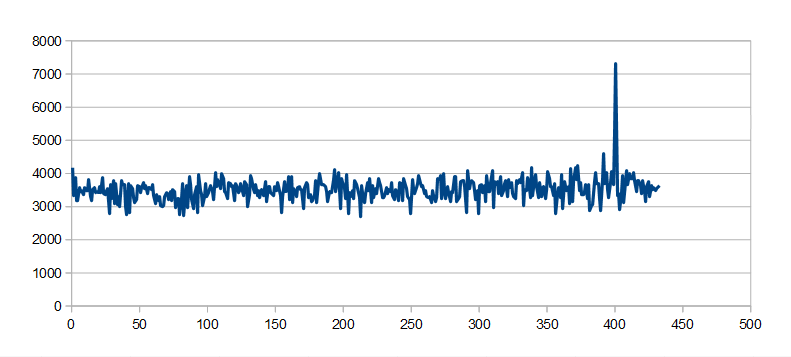
\includegraphics[scale=0.75]{content/images/Experiment/DayCollection}
        \caption{Collection times of the measurements from 03:30h to 04:00h}
        \label{fig:dayC}
    \end{subfigure}
    \caption{}
\end{figure}